

\section{Как я вижу программистов}
\showTOC


\begin{frame}[t,fragile]{Идея №1: давай распараллелим!}
\framesubtitle{Обычно бывает так}

Коллега предлагает переписать часть проекта с использованием нескольких потоков

\end{frame}


\begin{frame}[t,fragile,noframenumbering]{Идея №1: давай распараллелим!}
\framesubtitle{Обычно бывает так}

Коллега предлагает переписать часть проекта с использованием нескольких потоков

\begin{tikzpicture}[remember picture,overlay]
\node[xshift=3cm,yshift=-1.5cm] at (current page.center) {
\includegraphics[width=.3\textwidth]{production/fry-easy.jpg}};
\end{tikzpicture}

\pause

Проходит время ...

\pause

\begin{itemize}
  \item Стало медленнее
  \pause
  \item Зависает
\end{itemize}

\end{frame}


 \begin{frame}[t,fragile,noframenumbering]{Идея №1: давай распараллелим!}
 \framesubtitle{Обычно бывает так}
 
 Коллега предлагает переписать часть проекта с использованием нескольких потоков
 
 \begin{tikzpicture}[remember picture,overlay]
 \node[xshift=3cm,yshift=-4.35cm] at (current page.center) {
\includegraphics[width=.3\textwidth]{production/fry-easy.jpg}};
 \end{tikzpicture}
 
 Проходит время ...
 
 \begin{itemize}
   \item Стало медленнее
   \item Зависает
   \item Код непонятный
 \end{itemize}
 
 \end{frame}


\begin{frame}[t,fragile,noframenumbering]{Идея №1: давай распараллелим!}
\framesubtitle{Обычно бывает так}

Коллега предлагает переписать часть проекта с использованием нескольких потоков

\begin{tikzpicture}[remember picture,overlay]
\node[xshift=3cm,yshift=-4.0cm] at (current page.center) {
\includegraphics[width=.2\textwidth]{production/devil-latest.png}};
\end{tikzpicture}


Проходит время ...

\begin{itemize}
  \item Стало медленнее
  \item Зависает
  \item Код непонятный
\end{itemize}

\end{frame}


\begin{frame}[t,fragile]{Идея №1: давай распараллелим!}
\framesubtitle{Почему так происходит?}

\pause

 \begin{tabular}{p{0.5\textwidth} p{0.5\textwidth}}
 \begin{minted}[fontsize=\small]{java}
 synchronized(objectA) {
  synchronized(objectB) {
    computeStuff();
  }
 }
 \end{minted}
 
 & 
 
 \begin{minted}[fontsize=\small]{java}
 synchronized(objectB) {
  synchronized(objectA) {
    computeStuff();
  }
 }
 \end{minted}
 \end{tabular}

\pause 
Легко сломать многопоточную систему неаккуратным изменением.

\pause
Это ВСЕГДА случается после написания оригинального кода.

\pause

\begin{tikzpicture}[remember picture,overlay]
\node[xshift=-4cm,yshift=-6.0cm] at (current page.center) {
\includegraphics[width=.4\textwidth]{production/kiss/kiss.png}};
\node[xshift=3cm,yshift=-6.0cm] at (current page.center) {
\includegraphics[width=.35\textwidth]{production/kiss/1-prof-kiss.jpg}};
\end{tikzpicture}

\end{frame}


\begin{frame}[t]{Идея №1: давай распараллелим!}
\framesubtitle{Выводы}

Параллелизм полезен, но многопоточность приносит с собой:
\begin{itemize}
  \item Риски
  \item Издержки на поддержку
\end{itemize}

\pause
Реакция VM-инженера: изыди! Не хочу отлаживать этот код через полгода, после серии несвязанных правок, когда ты уже уволишься.

\pause
Реакция здорового человека: давай подумаем, стоит ли оно того.

\end{frame}


\begin{frame}[t]{Идея №2: давай по книжке сделаем!}
\framesubtitle{Взгляд VM-инженера}

\begin{tabular}{p{0.5\textwidth} p{0.5\textwidth}}  
\centering{Реальность} & 
\end{tabular}

\begin{tikzpicture}[remember picture,overlay]
\node[xshift=-3.2cm,yshift=-7.5cm] at (current page.center) {
\includegraphics[width=.35\textwidth]{production/art-cover.jpg}};
\end{tikzpicture}

\end{frame}


\begin{frame}[t,noframenumbering]{Идея №2: давай по книжке сделаем!}
\framesubtitle{Взгляд VM-инженера}

\begin{tabular}{p{0.5\textwidth} p{0.5\textwidth}}  
\centering{Реальность} & \centering{Мои ощущения}
\end{tabular}

\begin{tikzpicture}[remember picture,overlay]
\node[xshift=-3.2cm,yshift=-7.5cm] at (current page.center) {
\includegraphics[width=.35\textwidth]{production/art-cover.jpg}};
\end{tikzpicture}

\begin{tikzpicture}[remember picture,overlay]
\node[xshift=3.2cm,yshift=-7cm] at (current page.center) {
\includegraphics[width=.3\textwidth]{production/maniac-book.png}};
\end{tikzpicture}

\end{frame}


\begin{frame}[t]{Идея №2: давай по книжке сделаем!}
\framesubtitle{KSUH lock}

“A Fair Fast Scalable Reader-Writer Lock “, 1993

\begin{itemize}
  \item Orran \textbf{K}rieger, Michael \textbf{S}tumm, Ron \textbf{U}nrau, Jonathan \textbf{H}anna
  \item In Proc. of the International Conference on Parallel Processing

  \pause
  \item реализовано на языке Си

  \pause
  \item алгоритм формализован на языке Promela и верифицирован инструментом SPIN % TODO-link, TODO-footnote верифицирован частично

\end{itemize}

\pause

“Using Hardware Transactional Memory to Correct and Simplify and Readers-writer Lock Algorithm”, 2013
\begin{itemize}

  \pause
  \item 20 лет спустя!

  \pause
  \item Обнаружена ошибка в алгоритме, связанная с управлением памятью. Проявлялась на реальной системе.
\end{itemize}

\end{frame}


\begin{frame}[t,noframenumbering]{Идея №2: давай по книжке сделаем!}
\framesubtitle{KSUH lock}

“A Fair Fast Scalable Reader-Writer Lock “, 1993

\begin{itemize}
  \item Orran \textbf{K}rieger, Michael \textbf{S}tumm, Ron \textbf{U}nrau, Jonathan \textbf{H}anna
  \item In Proc. of the International Conference on Parallel Processing
  \item реализовано на языке Си
  \item алгоритм формализован на языке Promela и \textbf{верифицирован}\footnote{частично} инструментом SPIN
\end{itemize}

“Using Hardware Transactional Memory to Correct and Simplify and Readers-writer Lock Algorithm”, 2013
\begin{itemize}
  \item 20 лет спустя!
  \item Обнаружена ошибка в алгоритме, связанная с управлением памятью. Проявлялась на реальной системе.
\end{itemize}

\end{frame}


\begin{frame}[t]{Идея №2: давай по книжке сделаем!}
\framesubtitle{Выводы}

Сложные алгоритмы нужны, но приносят с собой:
\begin{itemize}
  \item Риски
  \item Издержки на поддержку
\end{itemize}


\pause
Реакция VM-инженера: ты точно понимаешь, что написано в книжке и почему оно будет работать?

\pause
Реакция здорового человека: неудобно, если для редактирования кода требуется кандидатская степень по распределенным системам. 

\pause

\includegraphics[width=.3\textwidth]{production/kiss/2-bender-kiss.png}


\begin{tikzpicture}[remember picture,overlay]
\node[xshift=2cm,yshift=-2.5cm] at (current page.center) {
\includegraphics[width=.4\textwidth]{production/kiss/kiss.png}};
\end{tikzpicture}

\end{frame}


\begin{frame}[t]{Идея №2: давай по книжке сделаем!}
\framesubtitle{Но если ты эксперт, то тогда можно?}

Промышленные системы быстры благодаря хитрым решениям.

\pause

\includegraphics[width=.3\textwidth]{production/super-duper.png}

\pause

\begin{tikzpicture}[remember picture,overlay]
\node[xshift=1.5cm,yshift=-1.5cm] at (current page.center) {
\includegraphics[width=.4\textwidth]{production/morbo.png}};
\end{tikzpicture}

\end{frame}


\begin{frame}[t,noframenumbering,fragile]{Идея №2: давай по книжке сделаем!}
\framesubtitle{Но если ты эксперт, то тогда можно?}

Промышленные системы быстры благодаря хитрым решениям.

Пример из Java-мира: biased locking.

\pause
Хитрая штука, чтобы ваши \textittt{synchronized} работали очень быстро\footnote<2->{\tiny\url{https://mechanical-sympathy.blogspot.com/2011/11/biased-locking-osr-and-benchmarking-fun.html}}.

\begin{minted}[fontsize=\small]{java}
while (0 != count--) {
  synchronized (jvmLock) {
    ++counter;
  }
}
\end{minted}

\pause
\begin{center}
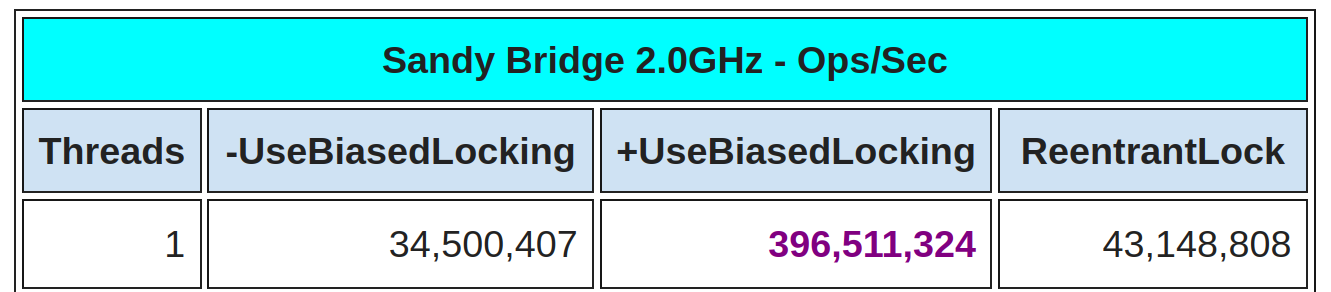
\includegraphics[width=.8\textwidth]{production/biased-locking.png}
\end{center}

\end{frame}


\begin{frame}[t,noframenumbering]{Идея №2: давай по книжке сделаем!}
\framesubtitle{Но если ты эксперт, то тогда можно?}

Промышленные системы быстры благодаря хитрым решениям.

Пример из Java-мира: biased locking.

\begin{itemize}
 \item Опубликован в 2006 году\footnote{\tiny\url{https://dl.acm.org/doi/10.1145/1167473.1167496}}

 \pause
 \item Служил верой и правдой

 \pause
 \item "Costly to maintain"

 \pause
 \item Deprecated в Java 15 (JEP 374, 2019)

\end{itemize}

\pause

\begin{tikzpicture}[remember picture,overlay]
\node[xshift=3.5cm,yshift=-5.5cm] at (current page.center) {
\includegraphics[width=.5\textwidth]{production/toad.jpeg}};
\end{tikzpicture}

\begin{tikzpicture}[remember picture,overlay]
\node[xshift=-3.5cm,yshift=-5.5cm] at (current page.center) {
\includegraphics[width=.4\textwidth]{production/kiss/kiss.png}};
\end{tikzpicture}

\end{frame}


\begin{frame}[t]{Идея №3: давай возьмем готовое!}
\framesubtitle{Хоть кто-то в состоянии написать сложную систему безошибочно?}

\pause 

\textttt{Linux futex\_wait() bug}\footnote<2->{\tiny\url{https://groups.google.com/g/mechanical-sympathy/c/QbmpZxp6C64/m/BonaHiVbEmsJ}}

\pause
Gil Tene (CEO of Azul, co-author of C4 GC):

\begin{quote}
  We had this one bite us hard and scare the \%\$\^\! out of us, so I figured I'd share the fear.
\end{quote}

\pause

\begin{quote}
The linux futex\_wait call has been broken for about a year.
\end{quote}

\pause

\begin{quote}
The impact of this kernel bug is very simple: user processes can deadlock and hang in seemingly impossible situations. Thread.park() in Java may stay parked.
\end{quote}

\pause

\begin{quote}
You'll spend a couple of months of someone's time trying to find the fault in your code, when there is nothing there to find. 
\end{quote}

\end{frame}


\begin{frame}[t,noframenumbering]{Идея №3: давай возьмем готовое!}
\framesubtitle{Хоть кто-то в состоянии написать сложную систему безошибочно?}

\begin{center}

\includegraphics[width=0.7\textwidth]{production/doom.jpg}
\end{center}

\end{frame}


\begin{frame}[t]{Идея №3: давай возьмем готовое!}
\framesubtitle{Выводы}

\begin{itemize}
  \item Выбирайте проверенные технологии
  \pause
  \item Регулярно обновляйтесь
  \pause
  \item Можете не использовать хитрые алгоритмы -- не используйте
\end{itemize}

\pause

\begin{center}

\includegraphics[width=.7\textwidth]{production/kiss/3-bart-kiss.jpg}
\end{center}

\end{frame}


% \begin{frame}{Идея №3: давай возьмем готовое!}
% 
% Василий прелагает взять библиотеку из репозитория со 100500 звездочек.
% Сотни опытнейших людей со всего мира обязательно вычитывают каждый коммит, и для нас сойдет.
% 
% Очки рантайма:
% Там import другим кеглем. Ну-ка
% Ага, import com.highway.to.hell
% 
% \end{frame}
% 
% 
% \begin{frame}{Идея №3: давай возьмем готовое!}
% 
% Пользоваться готовым надо уметь, в том числе читать непростые доки
% (MPSC не так использован, да еще присыпан неверным интерфейсом)
% 
% \end{frame}
% 
% \begin{frame}{Идея \#3: возьмем готовое!}
% 
% Ну, даже в стандартной библиотеке для Java есть "особенности"
% https://bugs.openjdk.org/browse/JDK-8256833
% [concurrency-interest] ConcurrentLinkedDeque is non-linearizable
% 
% В целом, надо думать всегда. Иногда "минимальный объем думания" для написания нормального кода весьма большой.
% 
% \end{frame}


\begin{frame}[t]{Как страшно жить}

\begin{center}
Жизнерадостный коллега 


\includegraphics[width=.4\textwidth]{production/sad-fry.png}

Почему так?

\end{center}
\end{frame}

\begin{frame}[t]{Почему так?}
\framesubtitle{Личный опыт}

Человеческий мозг не предназначен для многопоточности. 

\pause

Сложно представлять одновременное исполнение потоков и все возможные пересечения.

\pause

\begin{center}

\includegraphics[width=.6\textwidth]{production/crazy-prof.png}
\end{center}

\end{frame}
 
\begin{frame}[t]{Неконкретные советы}

Используйте
\begin{itemize}
  \item Простые решения

  \pause
  \item Готовые библиотеки для сложных стандартных задач

  \pause
  \item Шаблоны проектирования многопоточных систем

  \pause
  \item Предметно-ориентированные языки
\end{itemize}

\pause
\
\
\
\
\
\

А если меня беспокоит производительность?

\begin{tikzpicture}[remember picture,overlay]
\node[xshift=4.0cm,yshift=-5.5cm] at (current page.center) {
\includegraphics[width=.6\textwidth]{production/what-about-perf-2.png}};
\end{tikzpicture}

\end{frame}
 